\section{Anal\'yza} \label{sec:analyza}

\subsection{Anal\'yza protokolu IPFIX}

Protokol IPFIX - \emph{IP Flow Information Export} je IETF \emph{(Internet Engineering Task Force)}
štandard pre export informácií o sieťových tokoch zo smerovačov, meracích sond, 
alebo špecializovaných nástrojov. 
Aby bolo možné prenášať tieto informácie 
od exportovacieho procesu k zhromažďovaciemu procesu, je potrebný štandardizovaný 
spôsob komunikácie a taktiež jednotná reprezentácia odovzdávaných dát.
Protokol je vyvíjaný rovnomennou pracovnou skupinou \citep{ipfixCharter} od roku 2001 a 
vznikol ako priamy nasledovník proprietárneho protokolu Cisco Netflow Version 9 \citep{rfc3954}. 
To znamená, že IPFIX je založený na systéme výmeny informácií na základe šablón. To ho robí veľmi
flexibilným, pretože je možné nakonfigurovať, ktoré vlastnosti tokov sa majú merať.
Zjednodušená architektúra protokolu IPFIX je na Obrázku \ref{o:ipfix_architekture_basic}. 
\citep{rfc5101, ipfixProtocol, juvhaugen, veri}

\begin{figure}[ht!]
\centering
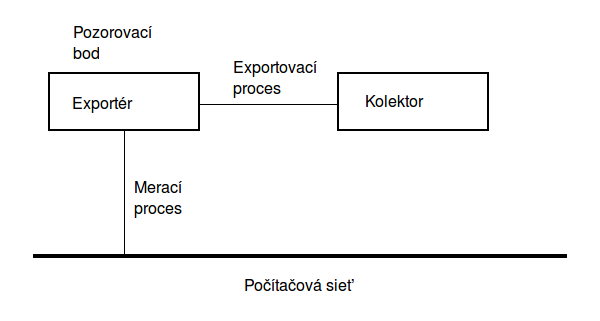
\includegraphics[width=0.7\textwidth]{ipfix_architekture_basic}
\caption{Zjednodušená verzia IPFIX architektúry}\label{o:ipfix_architekture_basic}
\end{figure}

\subsubsection{Terminológia} \label{sec:ipfix_terminology}

Podľa \citep{rfc3917} existuje veľa definícií termínu \uv{tok} používaných Internetovou komunitou.
Pracovná skupina IPFIX používa nasledujúcu:
\begin{description}
  \item[Tok] je definovaný ako množina IP paketov prechádzajúcich pozorovacím bodom v sieti, počas určitého 
časového intervalu. Všetky pakety patriace príslušnému toku majú množinu spoločných vlastností. Opačne 
môžeme tvrdiť, že každý paket patrí toku, ak spĺňa všetky tieto spoločné vlastnosti. 
\end{description}

Ďalšie termíny zavádza \citep{rfc5101}:
\begin{description}
  \item[Záznam o toku] obsahuje namerané informácie a charakteristické vlastnosti 
konkrétneho toku, ktorý bol pozorovaný pozorovacím bodom (napr. celkový počet prenesených 
bajtov, zdrojová IP adresa toku, a pod.).

  \item[Pozorovací bod] je miestom v sieti, kde sú IP pakety pozorované. Medzi príklady patrí 
sieťová linka, na ktorej je zavedená meracia sonda, zdieľané médium (napr. Ethernet LAN), 
alebo fyzické, či logické rozhranie smerovača. Každý pozorovací bod je asociovaný s 
pozorovacou doménou. 

  \item[Pozorovacia doména] je množina pozorovacích bodov. Je identifikovaná číslom 
(Observation Domain ID), ktoré je unikátne v rámci exportovacieho procesu. 

  \item[Merací proces] vytvára záznamy o tokoch na základe hlavičiek paketov. Vykonáva 
rôzne funkcie ako napríklad odchytávanie hlavičiek paketov, vytváranie časových známok, 
vzorkovanie, klasifikovanie a údržba záznamov o tokoch. 

  \item[Exportovací proces] odosiela záznamy o tokoch zhromažďovacím 
procesom. Tieto záznamy sú generované jedným alebo viacerými meracími procesmi.
	
  \item[Exportér] odosiela dáta o tokoch. Je to nástroj ktorý zastrešuje exportovacie procesy.

  \item[Kolektor] je nástroj, ktorý prijíma dáta od exportéra. Pozostáva z jedného, alebo
viacerých zhromažďovacích procesov.

  \item[Zhromažďovací proces] prijíma záznamy o tokoch od jedného, alebo viacerých 
exportovacích procesov. Prijaté záznamy môže spracovávať, alebo uchovávať. 

  \item[Informačné elementy] sú protokolovo nezávislým popisom atribútov záznamov o tokoch. 
Informačný model IPFIX \citep{rfc5102} obsahuje základnú množinu informačných elementov, vrátane ich
popisu, významu, dátového typu a pod. Informačné elementy sú rozdelené do 12 skupín, pozri Tabuľku \ref{t:ie-table},
na základe ich sémantiky a použitia. Každý element je asociovaný s dátovým typom, ktorý určuje jeho 
formát a spôsob kódovania.
Na základe tohto modelu sú jednotlivé dátové záznamy kódované na strane exportéra a dekódované 
v kolektore.
Informačný model povoľuje aj jeho rozširovanie. Organizácie môžu definovať vlastné informačné
elementy, ktorým musia prideliť unikátny identifikátor. 
Tieto elementy navyše obsahujú identifikátor organizácie \emph{(PEN)}, ktorý musí byť registrovaný v 
IANA\footnote{http://www.iana.org/assignments/enterprise-numbers}.

% ---- tabulka ----
\tabcolsep=8pt
\begin{table}[!ht]\caption{Základné skupiny informačných elementov podla \citep{rfc5102}}\label{t:ie-table}
\smallskip
\centering
\begin{tabular}{|c|c|}
\hline
\textbf{\#} & \textbf{názov skupiny} \\ \hline
1. & Identifikátory \\ \hline
2. & Konfigurátory meracieho a exportovacieho procesu \\ \hline
3. & Štatistické hodnoty meracieho a exportovacieho procesu \\ \hline
4. & Polia IP hlavičky \\ \hline
5. & Polia transportnej hlavičky \\ \hline
6. & Polia ostatných hlavičiek \\ \hline
7. & Odvodené vlastnosti paketov \\ \hline
8. & Min/Max vlastnosti tokov \\ \hline
9. & Časové známky tokov \\ \hline
10. & Počítadla vlastností tokov \\ \hline
11. & Rôzne vlastnosti tokov \\ \hline
12. & Výplň \emph{(padding)} \\ \hline
\end{tabular}
\end{table}

% -----------

\clearpage
  \item[Šablóna] špecifikuje formát odosielaných záznamov o tokoch pomocou zoznamu 
informačných elementov. Musí byť odoslaná kolektoru 
z exportovacieho procesu ešte pred odoslaním samotných dát. Neskôr sú šablóny periodicky 
preposielané, aby kolektor vedel v každom okamihu aký formát dát prijme. 
Šablóny musia byť dostupné administrátorom, preto sú definované v konfiguračnom súbore 
exportéra.
\citep{juvhaugen}
\end{description}



\subsubsection{Formát IPFIX správ} \label{sec:message_format}

Formát správ je definovaný v Špecifikácii IPFIX Protokolu \citep{rfc5101}. Správa pozostáva z 
hlavičky, nasledovaná niekoľkými IPFIX sadami. 
Exportér musí zakódovať všetky časti správy v sieťovom poradí bajtov (Big-Endian).
Na Obrázku \ref{o:ipfix_message_format} je jedna z možností formátu IPFIX správy. Za hlavičkou nasleduje sada šablón, pretože
šablóny musia byť exportované ihneď po vytvorení. Za šablónami nasledujú dátové sady a sady šablón možností 
v akomkoľvek poradí.

\begin{figure}[ht!]
\centering
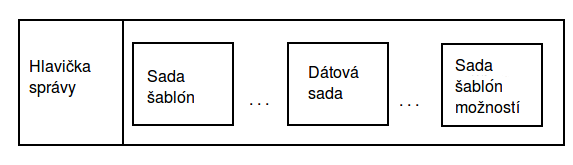
\includegraphics[width=0.7\textwidth]{ipfix_message_format}
\caption{Príklad formátu IPFIX správy}\label{o:ipfix_message_format}
\end{figure}



\paragraph{Formát hlavičky správy}

Formát hlavičky správy je znázornený na Obrázku \ref{o:ipfix_message_header}. Pozostáva z piatich poli:
\begin{itemize}
 \item \textbf{Číslo verzie} záznamu toku v správe. Pre IPFIX je to hodnota \verb|0x000a|.
 \item \textbf{Dĺžka} predstavuje celkovú dĺžku IPFIX správy v oktetoch, vrátane hlavičky a sád. 
 \item \textbf{Čas exportu} vo formáte UNIX timestamp. 
 \item \textbf{Sekvenčné číslo} vyjadruje počet odoslaných záznamov dátových záznamov modulo $2^{32}$  
 exportovacím procesom v tejto transportnej relácii. Túto hodnotu používa kolektor na odhalenie chýbajúcich 
 správ resp. dátových šablón.
 \item \textbf{Identifikačné číslo pozorovacej domény}, ktorý je lokálne jedinečný pre exportovací proces.
 \end{itemize}
 
\begin{figure}[ht!]
\centering
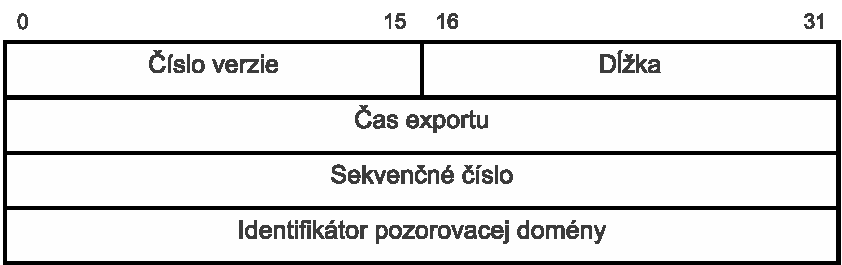
\includegraphics[width=0.7\textwidth]{ipfix_message_header}
\caption{Formát hlavičky IPFIX správy}\label{o:ipfix_message_header}
\end{figure}



\paragraph{Formát sady}

V IPFIX terminológii je sada všeobecný pojem pre kolekciu záznamov s podobnou štruktúrou. 
IPFIX správa môže obsahovať tri rôzne druhy sád:
\begin{itemize}
 \item Sada šablón,
 \item Dátová sada,
 \item Sada šablón možností.
\end{itemize}
Každá zo sád sa skladá z hlavičky sady a jedného, alebo viacerých záznamov sady, Obrázok \ref{o:set_format}. 
Na úplnom konci môže byť vložená výplň \emph{(padding)}, no nie je to povinná súčasť sady. Exportovací proces ho pridáva 
iba v tom prípade, keď chce aby sada bola zarovnaná na dĺžku, ktorá je násobkom 4, alebo 8.

\begin{figure}[ht!]
\centering
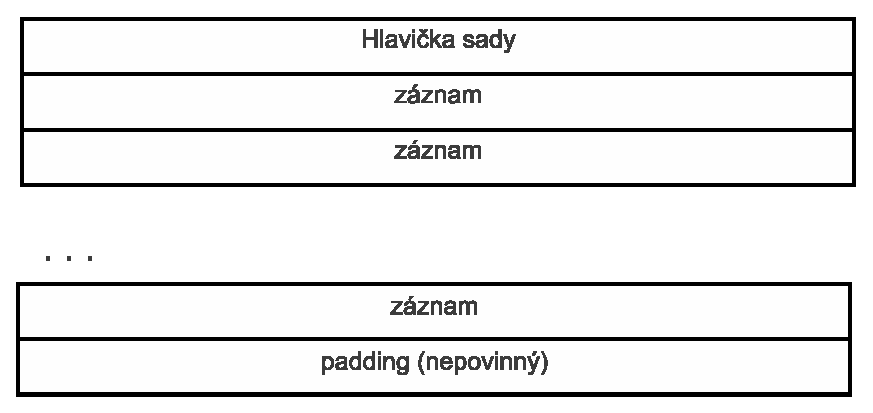
\includegraphics[width=0.7\textwidth]{set_format}
\caption{Formát sady}\label{o:set_format}
\end{figure}

\textbf{Hlavička sady} je rovnaká pre všetky tri typy sád. Je zobrazená na Obrázku \ref{o:set_header}. 
\emph{Identifikátor sady} určuje typ sady a teda aj typ všetkých záznamov obsiahnutých v sade, pozri 
Tabuľku \ref{t:set-record}. 
Sada istého druhu nemôže obsahovať záznamy iného typu. 
Hodnota 2 je rezervovaná pre sadu šablón. Sada šablón možností nadobúda 
hodnotu 3. Identifikátory 0 a 1 sa nepoužívajú z historických dôvodov \citep{rfc3954} a hodnoty od 4 po 
255 sú rezervované pre budúce použitie. Dátové sady sú označené hodnotami väčšími ako 255. 


\begin{figure}[ht!]
\centering
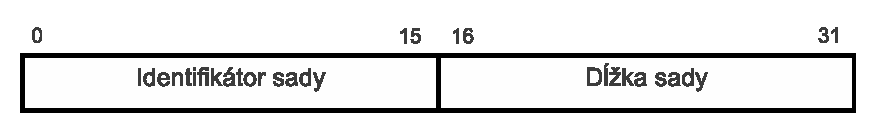
\includegraphics[width=0.7\textwidth]{set_header}
\caption{Formát hlavičky sady}\label{o:set_header}
\end{figure}

\emph{Dĺžka sady} zahŕňa celkovú dĺžku všetkých sád, vrátane hlavičky sady a prípadne výplne. Na jej základe 
sa určuje koniec tejto sady a začiatok ďalšej, pretože sada môže obsahovať rôzny počet záznamov.

% ---- tabuľka ----
\tabcolsep=8pt
\begin{table}[!ht]\caption{Prehľad identifikátorov, typov a záznamov sady}\label{t:set-record}
\smallskip
\centering
\begin{tabular}{|c|c|c|}
\hline
\textbf{Identifikátor sady} & \textbf{typ sady} & \textbf{typ záznamov} \\ \hline
0 - 1 & -- & -- \\ \hline
2 & sada šablón & záznamy šablóny \\ \hline
3 & sada šablón možností & záznamy šablóny možností \\ \hline
4 - 255 & -- & -- \\ \hline
255 - 65535 & dátová sada & dátové záznamy \\ \hline
\end{tabular}
\end{table}
% -----------


\paragraph{Špecifikátory poľa}

Špecifikátor poľa je akousi obálkou nad informačným elementom, Obrázok \ref{o:field_specifier_format}, 
vďaka nemu vie zhromažďovací proces spracovávať prijaté dáta. 

Prvý bit sa nazýva \emph{Enterprise bit}.
Ak je nastavený na 0, tak hovoríme o oficiálnom informačnom elemente charakterizovanom organizáciou IETF a 
registrovanom v IANA. 
V tomto prípade je \emph{číslo organizácie (PEN)} nevyplnené. V opačnom prípade, 
keď je tento bit nastavený na 1, ide o organizáciou špecifikovaný informačný element a číslo organizácie
musí byť zadané. Laboratórium počítačových sietí na Technickej univerzite v Košiciach má pridelené číslo 
organizácie 26235 \citep{pen}.
Dĺžka poľa vyjadruje na koľkých oktetoch je daný informačný element kódovaný. 
Zoznam informačných elementov aj s ich dĺžkami je dostupný v \citep{rfc5102}.
Špeciálny prípad nastáva pri redukovanom kódovaní. Vtedy je dĺžka poľa menšia ako popisuje 
Informačný model. 
 
\begin{figure}[ht!]
\centering
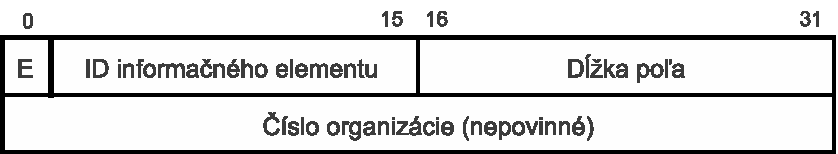
\includegraphics[width=0.7\textwidth]{field_specifier_format}
\caption{Formát špecifikátora poľa}\label{o:field_specifier_format}
\end{figure}



\paragraph{Formát záznamov šablóny}

Záznamy šablóny patria k nevyhnutným prvkom IPFIX správy. Na ich základe, a základe Informačného modelu
IPFIX \citep{rfc5102} vie zhromažďovací proces dekódovať dátové záznamy.
Šablóny môžu obsahovať akúkoľvek kombináciu informačných elementov. Či už oficiálnych -- navrhnutých 
spoločnosťou IANA, alebo vlastných -- vytvorených organizáciami.

Záznam šablóny tvorí \emph{hlavička}, pozri Obrázok \ref{o:template_record_header}, nasledovaná 
\emph{špecifikátormi poľa}. 
Každá šablóna musí mať v rámci transportnej relácie a pozorovacej domény jedinečný \emph{identifikátor}. 
Čísluje sa od 255 do 65535, rovnako ako identifikátory dátových sád, pretože každá šablóna referuje 
na dátovú sadu, ktorej štruktúru popisuje. \emph{Počet polí} sa týka počtu 
špecifikátorov poľa.

\begin{figure}[ht!]
\centering
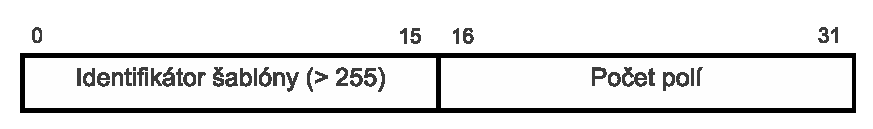
\includegraphics[width=0.7\textwidth]{template_record_header}
\caption{Formát hlavičky záznamu šablóny}\label{o:template_record_header}
\end{figure}



\paragraph{Formát záznamov šablóny možností}

Tieto záznamy dávajú exportéru možnosť poskytnúť kolektoru dodatočné informácie o kontexte posielaných dát, 
ktoré by zo samotných 
záznamov tokov nevedel vyčítať. Príkladom týchto informácií sú kľúče tokov, alebo konfigurácia šablóny,
vzorkovacie parametre a pod.

Formát záznamov (Obrázok~\ref{o:options_record_header}) je podobný ako v prípade záznamov šablóny. Pozostáva z hlavičky záznamu 
a jedného, alebo viacerých špecifikátorov poľa. Formát špecifikátorov je rovnaký ako pri záznamoch šablóny.
Hlavička naviac obsahuje \emph{počet polí pôsobnosti}. Pôsobnosť charakterizuje kontext 
informácií. Šablóna povoľuje 
definovať viac polí pôsobnosti ako jedno. V tomto prípade je celková pôsobnosť daná kombináciou týchto polí.
Počet polí pôsobnosti nemôže byť nulový, pričom \emph{počet polí} je 
súčtom polí pôsobnosti a špecifikátorov poľa.\citep{rfc5102}

\begin{figure}[ht!]
\centering
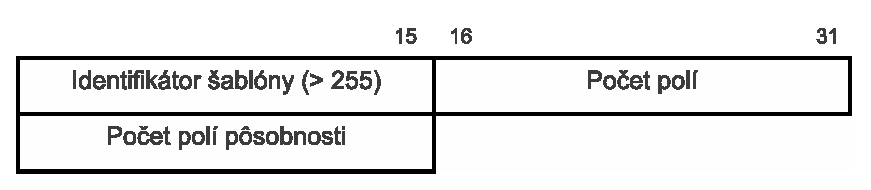
\includegraphics[width=0.7\textwidth]{options_record_header}
\caption{Formát hlavičky záznamu šablóny možností}\label{o:options_record_header}
\end{figure}



\paragraph{Formát dátových záznamov}

Dátové záznamy sú posielané v dátových sadách. Ich formát je veľmi 
jednoduchý. Pozostávajú len z hodnôt polí, nemajú ani vlastnú hlavičku. 
Sú kódované podla popisu v Informačnom modeli \citep{rfc5102}. Identifikátor 
šablóny, ktorá popisuje tieto hodnoty je zakódovaný v hlavičke sady, v časti
identifikátor sady. Inými slovami \uv{identifikátor sady} = \uv{identifikátor 
šablóny}. Aby vedel kolektor tieto dáta dekódovať, musí poznať formát šablóny 
už pred prijatím prvého dátového záznamu.

\subsection{Anal\'yza sprostredkovania spr\'av v IPFIX}

Výhodou monitorovania sieťovej prevádzky na báze tokov je to, že je možné merať 
veľké množstvo sieťovej prevádzky v distribuovaných pozorovacích bodoch. 
Zatiaľ čo tento typ monitorovania môže byť použitý na rôzne účely a pre rozmanité aplikácie, je veľmi 
obtiažne aplikovať ho paralelne na viac aplikácii s veľmi rozdielnymi požiadavkami.
Sieťoví administrátori musia nastaviť parametre meracích nástrojov tak, aby vyhoveli požiadavkám každej
jednej monitorovacej aplikácii. Takéto konfigurácie často nie sú podporované meracími nástrojmi. Či už
kvôli funkčným obmedzeniam, alebo kvôli pamäťovým a výpočtovým limitom, ktoré zamedzujú meraniu veľkých 
dátových tokov. Sprostredkovanie správ v IPFIX - \emph{IP Flow Information Export (IPFIX) Mediation}
vypĺňa túto medzeru medzi obmedzenými možnosťami merania a požiadavkami na monitorovacie aplikácie 
zavedením sprostredkovateľského zariadenia nazývaného \emph{IPFIX Mediátor} \citep{rfc5982}.

\subsubsection{Terminológia}
Terminológia použitá v tejto kapitole je čiastočne definovaná v podkapitole \ref{sec:ipfix_terminology} 
na strane \pageref{sec:ipfix_terminology}. 
Dodatočne zadefinujeme nasledujúce termíny:
\begin{description}
 \item[Prúd záznamov] - \emph{record stream} je sled dát nesúcich informácie o tokoch.
 
 \item[Sprostredkovanie správ v IPFIX] - \emph{IPFIX Mediation} je manipulácia a konverzia prúdu záznamov
 pomocou IPFIX protokolu.
 
 \item[Sprostredkovateľský proces] - \emph{Intermediate Process} prijíma prúd záznamov ako vstupnú 
 veličinu od zhromažďovacieho procesu, meracieho procesu, čítačky IPFIX súborov, iného 
 sprostredkovateľského zariadenia, alebo akéhokoľvek zdroja záznamov. Nad prijatými záznamami
 vykoná rôzne transformácie, na základe ich obsahu. Napokon zmenené záznamy posúva na svoj výstup buď
 smerom k exportovaciemu procesu, inému sprostredkovateľskému zariadeniu, alebo zapisovaču IPFIX súborov
 za účelom vykonania sprostredkovania IPFIX správ.
 
 \item[IPFIX Mediátor] je nástroj vykonávajúci sprostredkovanie správ tak, že prijíma prúd záznamov 
 z rôznych dátových zdrojov, zastrešuje jeden alebo viac sprostredkovateľských procesov  
 aby modifikoval obsah prúdu a nakoniec exportuje pozmenené dáta vo forme IPFIX správ pomocou exportovacieho
 procesu. V typickom prípade prijíma Mediátor prúd záznamov od zhromažďovacieho procesu. No rovnako môže
 prijímať údaje od iných zdrojov, ktoré nie sú zakódované pomocou IPFIX, napr. v prípade konverzie 
 protokolu NetFlow verzie 9 \citep{rfc3954} na IPFIX. Príklad jednej z možných architektúr, 
 v ktorej je použitý Mediátor je na obrázku \ref{o:exp_med_coll} \citep{rfc5982}.
\end{description}

\begin{figure}[ht!]
\centering
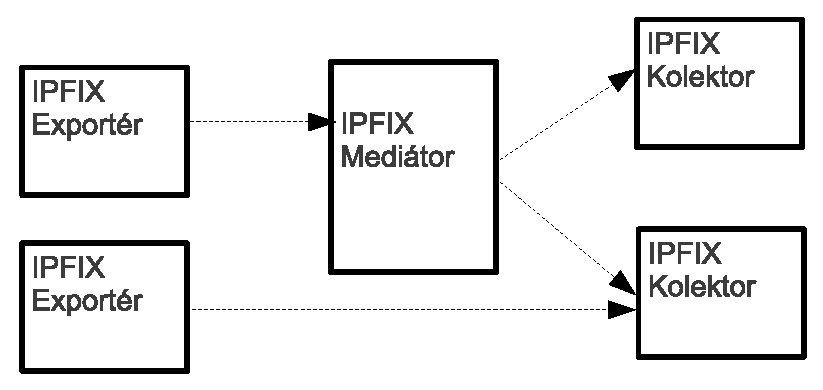
\includegraphics[width=0.7\textwidth]{exp_med_coll}
\caption{Príklad jednej z možných architektúr exportér - mediátor - kolektor}\label{o:exp_med_coll}
\end{figure}



\subsubsection{Anal\'yza nev\'yhod architekt\'ury bez Medi\'atora}


Problematika sprostredkovania IPFIX správ je podrobne spracovaná v \citep{rfc5982}. 
Hovori o tom, že sieťoví administrátori často celia problémom týkajúcim sa škálovateľnosti meracieho 
systému, flexibility monitorovania na základe tokov, alebo aj spoľahlivosti exportovania.
Napriek tomu, že sa vyvinuli známe techniky ako \emph{vzorkovanie a filtrovanie  paketov}, \emph{zoskupovanie 
dátových záznamov}, alebo \emph{replikácia exportu}, tieto problémy nevymizli.
Pozostávajú z prispôsobovania niektorých parametrov meracích nástrojov zdrojom meracieho 
systému zatiaľ čo musia naplniť patričné podmienky ako sú \emph{presnosť nameraných dát}, \emph{granularita 
toku}, či \emph{spoľahlivosť exportu}. Tieto okolnosti závisia na dvoch faktoroch:
\begin{enumerate}
 \item \textbf{Kapacita  meracieho systému} - pozostáva zo šírky pásma  spravovanej siete, kapacity 
 úložiska a výkonu exportovacích a zhromažďovacích nástrojov
 
 \item \textbf{Požiadavky aplikácie} - rôzne aplikácie vyžadujú rôznu zrnitosť záznamov o tokoch a presnosť dát.
\end{enumerate}



\paragraph{Vyrovnanie sa s rastom sieťovej prev\'adzky}

Veľké spoločnosti a poskytovatelia Internetového pripojenia (ISP) majú bežne vo svojej sieťovej 
infraštruktúre linky so šírkou pásma 10 Gb/s a ich celková sieťová prevádzka presahuje 100 Gb/s. 
Podla \citep{trafgrw} sieťová prevádzka používateľov širokopásmového pripojenia k
Internetu v blízkej budúcnosti sa bude každým rokom zvyšovať približne o 40\%. Sieťoví administrátori
monitorujúci IP prevádzku môžu udržiavať krok s týmto nárastom vďaka použitiu viacerých exportérov. 
Tento prístup však môže viesť k prekročeniu výpočtových a pamäťových možností jediného kolektora.

Tento problém zmierňujú redukčné techniky \emph{vzorkovanie a filtrovanie paketov} popísané v \citep{rfc5475}
implementované v exportéroch. Podobne agregácia meraných dát. Tieto techniky však majú aj svoje nevýhody. 
Môžu viesť k stratám malých tokov, nemožnosti odhalenia drobných zmien a anomálií v prenášaných dátach. 
Filtrovanie spôsobuje, že len podmnožina dátových záznamov je exportovaná.

Vzhľadom k týmto nedostatkom sa vyžaduje aby sa veľké meracie infraštruktúry nespoliehali na 
spomínané redukčné techniky.


\paragraph{Vyrovnanie sa s viacúčelovým meraním}

Rôzne monitorovacie aplikácie majú rôzne požiadavky na meraciu infraštruktúru. Niektoré vyžadujú 
monitorovanie na úrovni tokov, iné informácie o individuálnych paketoch a ďalšie agregované toky a pod.

Ak by mal exportér naplniť tieto požiadavky, musel by paralelne vykonávať rôzne meracie operácie, čo je
kvôli limitovaným výpočtovým zdrojom takmer nemožné. Preto je výhodnejšie použiť exportér s jednoduchším a 
výkonnejším nastavením a namerané dáta vhodne spracovávať na ďalšej úrovni meracej architektúry.



\paragraph{Vyrovnanie sa s heterogénnym prostredím}

Administrátori môžu použivať IPFIX nástroje od rozmanitých výrobcov, s rozdielnymi verziami softvéru a s 
rôznymi typmi sieťových zariadení (smerovač, prepínač, meracia sonda) v jednej sieťovej doméne.
V niektorých topológiách sú stále nasadené historické protokoly na export tokov. Dosiahnutie plnej 
interoperability týchto zariadení nie je možné.

Monitorovací systém sa vie vysporiadať s týmto problémom iba keď je prítomné sprostredkovanie IPFIX správ.
Avšak obsiahnuť sprostredkovanie vo všetkých zhromažďovacích zariadeniach je náročné.


\paragraph{Zhrnutie problémov}

Vzhľadom k limitovaným zdrojom monitorovacieho systému, je dôležité použiť techniky redukcie sieťových 
dát čím nižšie v hierarchii systému, teda v exportéri. Avšak implementácia tohto návrhu je sťažená v 
heterogénnom prostredí exportovacích nástrojov. 
Na druhej strane, udržovanie presnosti dát a granularity tokov tak, aby boli splnené požiadavky 
rôznych monitorovacích aplikácii vyžaduje škálovateľnú a flexibilnú zhromažďovaciu infraštruktúru.

Toto zhrnutie implikuje, že nové sprostredkovateľské funkcie sú potrebné v typických exportér - kolektor
infraštruktúrach. 


\subsubsection{Vybrané príklady použitia sprostredkovania správ} \label{sec:mediator_examples}


RFC 5982 \citep{rfc5982} uvádza viacero príkladov zaradenia IPFIX Mediátora do klasickej
exportér - kolektor architektúry. Uveďme aspoň niektoré.


\paragraph{Prispôsobovanie granularity tokov}

Najzákladnejšia sada kľúčov toku je pätica: \emph{protokol}, \emph{zdrojová a cieľová IP adresa}, 
\emph{číslo zdrojového a cieľového portu}. Menšie sady kľúčov, teda trojice, dvojice, alebo len jeden 
samotný prvok (napr. \emph{maska siete}, \emph{BGP čísla autonómnych systémov}, a pod.) vytvárajú viac 
agregované záznamy o tokoch. Toto je vhodné pri meraní na úrovni 
jadra sieťovej domény, alebo pri manipulovaní s výkonnosťou exportérov a kolektorov.

Najvhodnejšia implementácia predstavuje konfigurovateľný merací proces v exportéri. Administrátor 
špecifikuje požadovanú sadu kľúčov toku a tým pádom exportér generuje záznamy o toku želanej zrnitosti.

V opačnom prípade, kde merací proces nemá schopnosť nastavovať kľúče toku exportéra, IPFIX Mediátor 
môže agregovať dátové záznamy na základe definovaných kľúčov vo svojej konfigurácii.


\paragraph{Distribuovaná zhromažďovacia infraštruktúra}

Zvyšovanie počtu IPFIX exportérov, rast objemu IP dát a rôzne požiadavky na operácie vykonávané nad 
dátovými záznamami v kolektore spôsobujú vysokú náročnosť na implementáciu všetkých meracích
aplikácii v rámci jedného kolektora.

Za účelom navýšenia zhromažďovacej kapacity resp. objemu spracovania dátových záznamov musia byť 
nasadené distribuované kolektory čím bližšie ku exportérom. V tomto prípade sa kolektory stanú 
IPFIX Mediátormi, ktoré budú preposielať dátové záznamy podľa požiadaviek centralizovaným aplikáciam.


\paragraph{Spájanie času}

Spájanie resp. kompozícia času je definovaná ako agregácia za sebou idúcich dátových záznamov s rovnakými
kľúčmi toku. Tento proces vedie k rovnakému výstupu ako nastavenie dlhšieho aktívneho timeoutu
\emph{(active timeout)} v exportéri, no má jednu výhodu. Nové metriky ako napríklad výpočet priemerných, 
maximálnych, alebo minimálnych hodnôt zo záznamov o tokoch v kratších časových intervaloch umožňujú 
presnejšie výsledky a sledovanie aj menších zmien.

Jedna z možných implementácii je použitie sprostredkovateľského procesu umiestneného medzi 
meracím a exportovacím procesom exportéra. Druhou možnosťou je samostatný IPFIX Mediátor situovaný medzi
exportérom a kolektorom. Táto možnosť prináša väčšiu flexibilitu a nezaťažuje exportér ďalšími výpočtami.


\paragraph{Spájanie priestoru} \label{sec:spatial}

Spájanie priestoru je vlastne zoskupenie dátových záznamov v rámci množiny pozorovacích bodov jednej 
pozorovacej domény, združovanie záznamov viacerých exportérov, alebo jedného exportéra ale viacerých 
pozorovacích domén. Delí sa na tieto štyri typy:

\begin{enumerate}
 \item \textbf{Spájanie priestoru v rámci jednej pozorovacej domény} \\ 
    Príkladom je meranie dátového toku jedného logického rozhrania, ktoré vzniklo agregáciou liniek 
    podla 802.3ad \citep{ieee802.3}.
 \item \textbf{Spájanie priestoru viacerých pozorovacích domén jedného exportéra} \\
    Tak isto ako v predchádzajúcom príklade aj tu ide o agregáciu viacerých fyzických liniek. 
 \item \textbf{Spájanie priestoru niekoľkých exportérov} \\
    Dátové záznamy namerané v rámci jednej administratívnej domény môžu byť zlučované.
 \item \textbf{Spájanie priestoru administratívnych domén} \\
    Dátové záznamy zaznamenané vo viacerých administratívnych doménach, ako napríklad v rôznych klientskych 
    sieťach, alebo v sieťach rozdielnych poskytovateľov Internetového pripojenia môžu byť tiež zlučované.
    Kolektor vie na základe IP adresy exportéra rozlíšiť, ktorej klientskej sieti exportér patrí a tak 
    rozlišovať klientske dáta.
\end{enumerate}

Implementácia pomocou sprostredkovateľského procesu umiestneného v exportéri rieši prípady 1 a 2. 
Separátny IPFIX Mediátor je riešením pre  všetky štyri prípady.


\paragraph{Anonymizácia dátových záznamov}

IPFIX exporty krížom cez administratívne domény, tak ako to bolo popísané v prípade 4 
v podkapitole \ref{sec:spatial}, na strane \pageref{sec:spatial} môžu 
byt použité na monitorovanie sieťovej prevádzky na veľké vzdialenosti, 
napríklad pre analýzu dátových trendov v Internete. Pri takomto použití sa musia administrátori riadiť
pravidlami pre ochranu súkromia a predísť monitorovaniu dôvernej sieťovej prevádzky cudzími osobami.
Typicky anonymizačné techniky umožňujú poskytovanie sieťových dát iným osobám bez porušenia týchto zásad.

Všeobecne platí, že anonymizácia upraví sadu dát tak, aby chránila identitu ľudí alebo subjektov, 
ktorých sa súbor dát týka. Zároveň sa pokúša zachovať dáta tak, aby boli stále zmysluplné pre danú 
analýzu ale súčasne nemôžu byť stopovateľné naspäť ku konkrétnym sieťam, pracovným staniciam, alebo 
používateľom generujúcim tieto dáta. Napríklad, anonymizácia IP adresy je veľmi dôležitá pre 
zamedzenie identifikácie užívateľov, alebo smerovačov. 

Jedným z možných prevedení v tomto prípade používa anonymizačnú funkciu v exportéri. 
To však príliš zvyšuje zaťaženie exportéra. Flexibilnejšia implementácia využíva samostatný 
IPFIX Mediátor medzi exportérom a kolektorom.


\paragraph{Distribúcia dátových záznamov}

Trendom v moderných dátových sieťach je súčasný prenos dát, hlasu a video komunikácie jednou 
spoločnou infraštruktúrou. Takéto siete nazývame konvergovanými sieťami. 
Počítačové siete paralelne prenášajú dáta viacerých protokolov ako napríklad
IPv4, IPv6, VPN, MPLS a pod. Dátové záznamy každého z týchto protokolov musia byť analyzované 
oddelene a z rôznych perspektív pre rôzne organizácie.

Jeden kolektor pokrývajúci všetky typy dátových záznamov sa môže stať úzkym hrdlom 
zhromažďovacej infraštruktúry. Preto je lepšie distribuovať dátové záznamy na základe ich 
typu viacerým kolektorom, čo má za následok rozloženie zátaže. Pod typom dátového 
záznamu máme na mysli napríklad typ sieťového protokolu, ktorým boli dáta prenášane. 

Jedna z možných implementácií v tomto prípade používa replikáciu IPFIX správy v exportéri 
pre viac kolektorov. Každý kolektor potom dekóduje tie dátové záznamy, ktoré jeho aplikácia
potrebuje. To však zvyšuje zaťaženie exportovacieho procesu a mrhanie šírkou pásma medzi
exportérom a kolektorom.

Sofistikovanejšie prevedenie používa sprostredkovateľský proces v exportéri, ktorý určuje, 
ktorému kolektoru sa dáta pošlú, v závislosti na hodnotách určitých polí. Ak exportér nemá
túto schopnosť, posiela dátové záznamy IPFIX Mediátoru, a ten ich distribuuje kolektorom.


\paragraph{Interoperabilita medzi protokolmi starších verzií a IPFIX}

Počas migrácie z protokolov starších verzií ako napríklad NetFlow \citep{rfc3954} na IPFIX
zvyknú nástroje týchto protokolov súčasne existovať v jednej sieti. Napríklad aj po zavedení 
IPFIX kolektora je nutné monitorovať sieť, hoci exportér je verzie NetFlow.

Jedna z možností je použiť IPFIX Mediátor, ktorý bude konvertovať starší protokol na IPFIX.



\subsubsection{Vybrané implementačno-špecifické problémy IPFIX Mediátora} \label{sec:problems}


\paragraph{Strata informácie o pôvodnom exportéri} \label{sec:loss_info}

Pri využívaní sprostredkovania správ v IPFIX dochádza k strate potrebných informácii. V prvom rade to je 
IP adresa exportéra, ktorá bola získavaná zo zdrojovej IP adresy transportnej relácie, rovnako 
ako identifikačné číslo pozorovacej domény, ktoré je zahrnuté v hlavičke IPFIX správy.
V niektorých prípadoch môže Mediátor zahodiť tieto informácie úmyselne. 
Vo všeobecnosti však platí, že kolektor musí rozpoznať pôvod nameraných dát, ako napríklad IP adresu 
exportéra, ID pozorovacej domény, alebo dokonca ID pozorovacieho bodu. Ak Mediátor tieto informácie 
o exportéri neoznámi kolektoru, tak ten nesprávne usúdi, že IP adresa Mediátora je adresa pôvodcu dát 
(exportéra).

V nasledujúcom obrázku \ref{o:loss_of_exporter} kolektor vie rozoznať dve IP adresy - 192.0.2.3. (Mediátor) 
a 192.0.2.2 (exportér 2). To nie je správne. Mediátor musí informovať kolektor o IP adrese exportéra 1.

\begin{figure}[ht!]
\centering
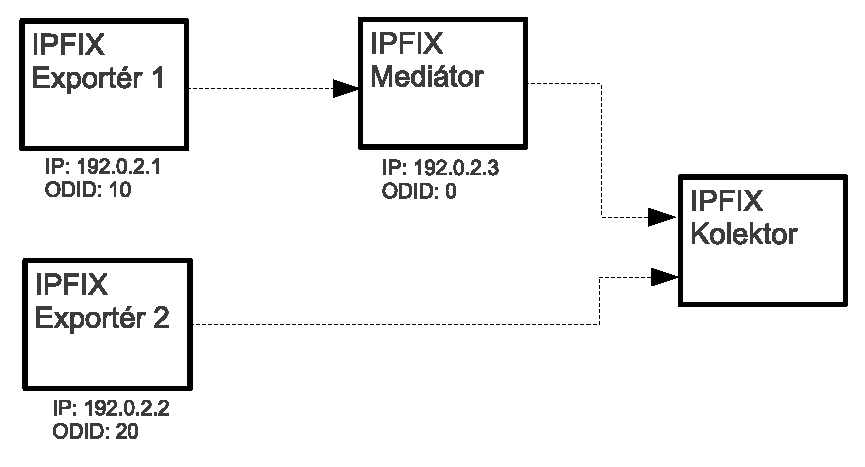
\includegraphics[width=0.7\textwidth]{loss_of_exporter}
\caption{Strata informácie o originálnom exportéri}\label{o:loss_of_exporter}
\end{figure}


\paragraph{Strata informácie o čase exportu} \label{sec:loss_time}

Pole čas exportu \emph{export time}, ktoré je zahrnuté v hlavičke správy predstavuje referenčnú 
časovú známku dátové záznamy. Niektoré informačné elementy popísané v \citep{rfc5102} nesú 
časové známky delta \emph{delta timestamps}, ktoré udávajú časový rozdiel voči hodnote v poli 
čas exportu. Ak dátový záznam zahŕňa nejaké pole s časovou známkou delta a Mediátor prepíše hodnotu 
času exportu,  tak časová známka delta týmto stráca význam. Kolektor však túto situáciu nevie 
rozpoznať a tak pracuje so zlými hodnotami.


\paragraph{Interpretácia sprostredkovaných správ}

V niektorých prípadoch potrebuje kolektor vedieť, ktoré konkrétne operácie resp. funkcie vykonal Mediátor 
nad dátovými záznamami. Kolektor nedokáže rozlíšiť medzi spájaním času a spájaním priestoru, v prípade, že 
Mediátor neexportuje použitú funkciu. Niektoré parametre vzťahujúce sa k funkcii by tiež mali byť 
exportované. 

V prípade spájania času, kolektor musí poznať aktívny timeout \emph{active timeout} 
pôvodných záznamov o tokoch. Pri spájaní priestoru je potrebné poznať nad akou oblasťou bola 
vykonaná kompozícia dátových záznamov.\citep{rfc5982}


